\documentclass[
    17pt,
    margin=1in,
    innermargin=-4.5in,
    blockverticalspace=-0.15in
]{tikzposter}
\geometry{paperwidth=42in,paperheight=30in}
\usepackage[utf8]{inputenc}
\usepackage{amsmath}
\usepackage{amsfonts}
\usepackage{amsthm}
\usepackage{amssymb}
\usepackage{mathrsfs}
\usepackage{graphicx}
\usepackage{subcaption}
\usepackage{adjustbox}
\usepackage{enumitem}
\usepackage{multirow}
\usepackage[american]{babel}
\usepackage{csquotes}
\usepackage{booktabs}
\usepackage{numprint}
\usepackage[backend=biber,style=apa]{biblatex}
\DeclareLanguageMapping{american}{american-apa}
\usepackage{emory-theme}
\usepackage{inconsolata} % very nice fixed-width font included with texlive-full
\usepackage{color} % more flexible names for syntax highlighting colors
\usepackage{listings}
\lstdefinelanguage{julia}
{
  keywordsprefix=\@,
  morekeywords={
    exit,whos,edit,load,is,isa,isequal,typeof,tuple,ntuple,uid,hash,finalizer,convert,promote,
    subtype,typemin,typemax,realmin,realmax,sizeof,eps,promote_type,method_exists,applicable,
    invoke,dlopen,dlsym,system,error,throw,assert,new,Inf,Nan,pi,im,begin,while,for,in,return,
    break,continue,macro,quote,let,if,elseif,else,try,catch,end,bitstype,ccall,do,using,module,
    import,export,importall,baremodule,immutable,local,global,const,Bool,Int,Int8,Int16,Int32,
    Int64,Uint,Uint8,Uint16,Uint32,Uint64,Float32,Float64,Complex64,Complex128,Any,Nothing,None,
    function,type,typealias,abstract
  },
  sensitive=true,
  morecomment=[l]{\#},
  morestring=[b]',
  morestring=[b]" 
}

\definecolor{mygray}{RGB}{128,128,128}
\definecolor{myblue}{RGB}{0, 0, 255}
\definecolor{myolivegreen}{RGB}{186, 184, 108}
\definecolor{mymaroon}{RGB}{128, 0, 0}

\lstset{
    language=julia,
    basicstyle=\ttfamily, 
    columns=fullflexible, % make sure to use fixed-width font, CM typewriter is NOT fixed width
    numbers=left, 
    numberstyle=\small\ttfamily\color{mygray},
    stepnumber=1,              
    numbersep=10pt, 
    numberfirstline=true, 
    numberblanklines=true, 
    tabsize=4,
    lineskip=-1.5pt,
    extendedchars=true,
    breaklines=true,        
    keywordstyle=\color{myblue}\bfseries,
    identifierstyle=, % using emph or index keywords
    commentstyle=\sffamily\color{myolivegreen},
    stringstyle=\color{mymaroon},
    showstringspaces=false,
    showtabs=false,
    upquote=false
}

\makeatletter
\newcounter{tablecounter}
\newenvironment{tikztable}[1][]{
  \def \rememberparameter{#1}
  \vspace{10pt}
  \refstepcounter{tablecounter}
  \begin{center}
  }{
    \ifx\rememberparameter\@empty
    \else
    \\[10pt]
    {\small Table.~\thetablecounter: \rememberparameter}
    \fi
  \end{center}
}
\makeatother

\usepackage{mwe}    % for placeholder images

\addbibresource{refs.bib}

% Set theme parameters
\tikzposterlatexaffectionproofoff
\usetheme{EmoryTheme}
\usecolorstyle{EmoryStyle}

\title{AdvancedHMC.jl: a modular implementation of Stan’s no-U-turn sampler in Julia}
\author{Kai Xu\textsuperscript{1}, Hong Ge\textsuperscript{2}, Will Tebbutt\textsuperscript{2}, Mohamed Tarek\textsuperscript{3}, Martin Trapp\textsuperscript{4} and Zoubin Ghahramani\textsuperscript{2,5}}
\institute{
    \textsuperscript{1}University of Edinburgh \quad \textsuperscript{2}University of Cambridge \quad \textsuperscript{3}UNSW Canberra \quad \textsuperscript{4}Graz University of Technology \quad \textsuperscript{5}Uber AI Labs
%    \textsuperscript{5}Austrian Research Institute for AI 
}
\titlegraphic{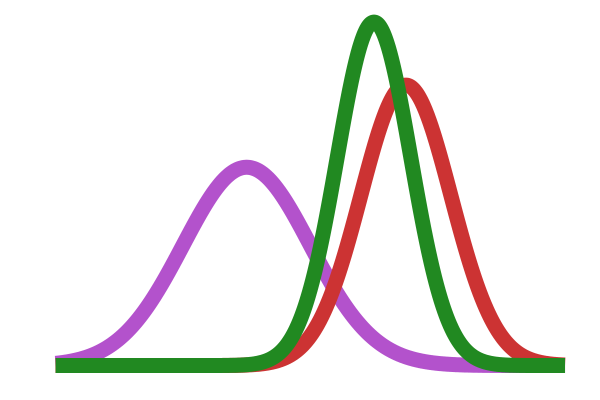
\includegraphics[width=0.075\textwidth]{turing-logo}}

% begin document
\begin{document}
\maketitle
\centering
\begin{columns}

\column{0.32}

\block{Abstract}{
    The No-U-Turn Sampler (NUTS) in \texttt{Stan} (\cite{hoffman2014no,carpenter2017stan}) has demonstrated remarkable sampling robustness and 
    efficiency in a wide range of Bayesian inference problems, 
    due to the use of dynamic Hamiltonian trajectory, 
    and a fine-tuned joint adaptation of step-size and mass matrix. 
    Motivated by these successes, we present 
    \texttt{AdvancedHMC.jl} (\texttt{AHMC}), a pure Julia implementation of \texttt{Stan}’s built-in NUTS algorithm and 
    related adaptation methods. 
    We hope \texttt{AdvancedHMC.jl} can help expose \texttt{Stan}’s NUTS to a wider range of users, 
    e.g. those who want to write their models by hand, 
    or using a different probabilistic programming language (e.g. \texttt{Turing}, \texttt{Soss}). 
    In our package, NUTS is defined as a combination of individual components with 
    abstractions 
%  including the `Hamiltonian` dynamics, the `Metric` space, 
%  how the dynamics are numerically simulated by an Integrator to build up a `Trajectory`, 
%  and how a candidate point is sampled from it by a `TrajectorySampler`. 
%  This abstraction is 
partially 
    inspired by 
    (\cite{betancourt2017conceptual}).
    % A Conceptual Introduction to Hamiltonian Monte Carlo” by Michael Betancourt.
}

\block{Hamiltonian Monte Carlo Components}{
    Hamiltonian Monte Carlo (HMC) simulates Hamiltonian dynamics to make proposals for a Markov chain (\cite{neal2011mcmc}).
    \texttt{AdvancedHMC.jl} supports various HMC samplers below.
    $$
    (\texttt{StaticHMC} \cup \texttt{DynamicHMC}) \times \texttt{Adaptor}.
    $$
    Here $\texttt{StaticHMC}$ are HMC with fixed-length trajectories and 
    $\texttt{DynamicHMC}$ are HMC with adaptive trajectory length 
    which can be created by composing NUTS components as follows
    $$
    \texttt{Metric} \times \texttt{Integrator} \times \texttt{TrajectorySampler} \times \texttt{TerminationCriterion},
    $$
    where 
    \begin{equation*}
        \begin{aligned} 
            \texttt{Metric} &=  \{ \texttt{UnitEuclidean}, \texttt{DiagEuclidean}, \texttt{DenseEuclidean} \} \\ 
            \texttt{Integrator} &=  \{ \texttt{Leapfrog} \} \\
            \texttt{TrajectorySampler} &=  \{ \texttt{Slice}, \texttt{Multinomial} \} \\
            \texttt{TerminationCriterion} &= \{ \texttt{ClassicNoUTurn}, \texttt{GeneralisedNoUTurn} \}
        \end{aligned}.
    \end{equation*}
    $\texttt{Adaptor}$ can be composed from base adaptors
    $$
    \texttt{BaseAdaptor} \in \{\texttt{Preconditioner}, \texttt{NesterovDualAveraging}\}.
    $$

    \textbf{Note 1}: $\texttt{Preconditioner}$ behaves differently based on the choice of metric spaces.

    \textbf{Note 2}: $\texttt{StanHMCAdaptor}$, a specific composition of base adaptors that is equivalent to \texttt{Stan}'s windowed adaptor, is provided. 
    This adaptor has been proved to be robust in practice.
}

\block{Benchmark Models}{
    We use five models from \texttt{MCMCBenchmarks.jl} to compare 
    NUTS between \texttt{AdvancedHMC.jl} and \texttt{Stan}. \\

    \textbf{Gaussian Model (Gaussian)}
    is a simple two parameter Gaussian distribution.
    $$
    \mu \sim \mathcal{N}(0, 1), \quad 
    \sigma \sim \mathcal{T}runcated(\mathcal{C}auchy(0, 5), 0, \infty), \quad
    y_n \sim \mathcal{N}(\mu, \sigma) \; (n = 1, \dots, N)
    $$
    
    \textbf{Signal Detection Model (SDT)}
    is a model used in psychophysics and signal processing, 
    which decomposes performance in terms of discriminability and bias.
    $$
    d \sim \mathcal{N}(0, \frac{1}{\sqrt{2}}), \quad 
    c \sim \mathcal{N}(0, \frac{1}{\sqrt{2}}), \quad 
    x \sim \text{SDT}(d, c)
    $$
    
    \textbf{Linear Regression Model (LR)}
    is a linear regression with truncated Cauchy prior on the weights.
    $$
    B_d \sim \mathcal{N}(0, 10), \;
    \sigma \sim \mathcal{T}runcated(\mathcal{C}auchy(0, 5), 0, \infty), \;
    y_n \sim \mathcal{N}(\mu_n, \sigma),
    $$
    where $\mu = B_0 + B^T X, d = 1, \dots, D$ and $n = 1, \dots, N$. \\
    
    \textbf{Hierarchical Poisson Regression (HPR)}
    $$
    a_0 \sim \mathcal{N}(0, 10), \;
    a_1 \sim \mathcal{N}(0, 1), \;
    b_\sigma \sim \mathcal{T}runcated(\mathcal{C}auchy(0, 1), 0, \infty), \;
    b_d \sim \mathcal{N}(0, b_\sigma), \;
    y_n \sim \mathcal{P}oi(\log\lambda_n),
    $$
    where $\log\lambda_n = a_0 + b_{z_n} + a_1 x_n, d = 1, \dots, N_b$ and $n = 1, \dots, N$. \\
    
    \textbf{Linear Ballistic Accumulator (LBA)}
    is a cognitive model of perception and simple decision making.
    $$
    \tau \sim \mathcal{T}runcated(\mathcal{N}(0.4, 0.1), 0, mn), \quad
    A \sim \mathcal{T}runcated(\mathcal{N}(0.8, 0.4), 0, \infty),
    $$
    $$
    k \sim \mathcal{T}runcated(\mathcal{N}(0.2, 0.3), 0, \infty), \quad
    \nu_d \sim \mathcal{T}runcated(\mathcal{N}(0, 3), 0, \infty), \quad
    x_n \sim \text{LBA}(\nu, \tau, A, k)
    $$
    where $mn=\min_i x_{i,2}, d = 1, \dots, N_c$ and $n = 1, \dots, N$.
}

\column{0.36}

\block{Example Code of Building \texttt{Stan}'s NUTS using \texttt{AHMC}}{
    \lstinputlisting{example.jl}
}

\block{Sampling Efficiency: \texttt{Stan}'s NUTS v.s. \texttt{AHMC}}{
    To compare the sampling efficiency between \texttt{Stan} and \texttt{AHMC},
    we run multiple runs of NUTS with target acceptance rate $0.8$ 
    for $2,000$ runs with $1,000$ adaptation steps,
    where the warm-up samples dropped.
    Below are figures of distributions of step size and tree depth,
    and the mean effective sample size (ESS) for different variables.
    \begin{tikzfigure}[Gaussian (50 runs); left to right: step size, tree depth, ESS]
        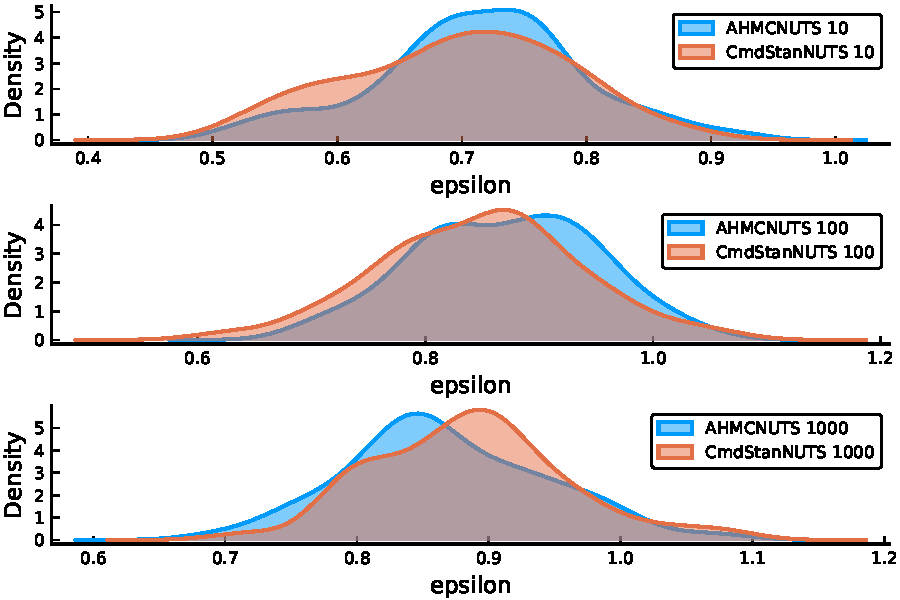
\includegraphics[width=0.08\textwidth]{./figs/Gaussian/density_epsilon.pdf}
        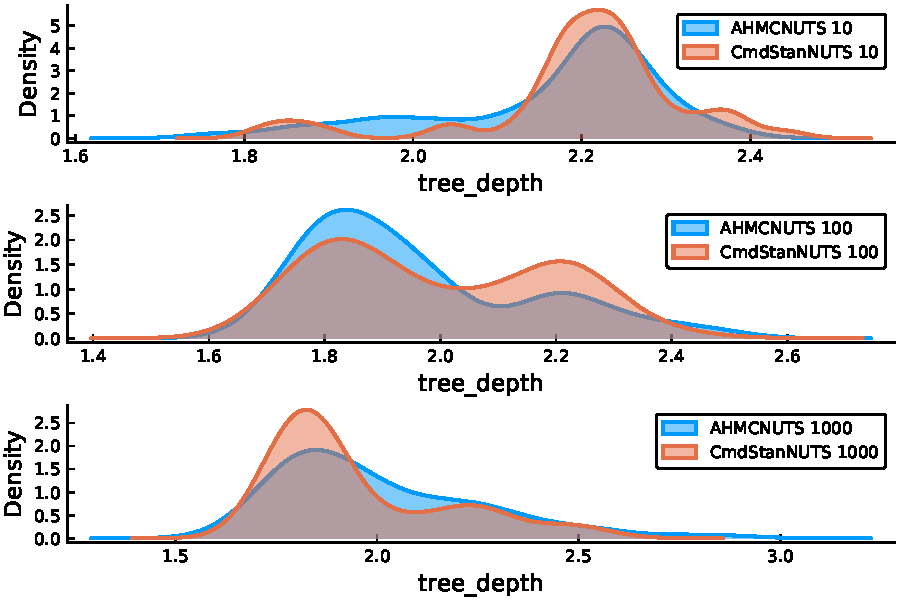
\includegraphics[width=0.08\textwidth]{./figs/Gaussian/density_tree_depth.pdf}
        \;\hfill
        \raisebox{\height}{\scalebox{0.75}{
            \begin{tabular}{lrrr}
                \toprule
                \multirow{2}{*}{} & \multirow{2}{*}{$N$} & \multicolumn{2}{c}{ESS} \\
                & & \multicolumn{1}{c}{$\mu$} & \multicolumn{1}{c}{$\sigma$} \\
                \midrule
                \texttt{Stan} & 10 & 513.163 & 466.577 \\
                \texttt{AHMC} & 10 & 503.535 & 447.722 \\
                \texttt{Stan} & 100 & 786.531 & 782.231 \\
                \texttt{AHMC} & 100 & 786.531 & 796.628 \\
                \texttt{Stan} & 1000 & 864.010 & 876.660 \\
                \texttt{AHMC} & 1000 & 832.255 & 844.452 \\
                \bottomrule
            \end{tabular}
        }}\hfill\;
    \end{tikzfigure}
    \vspace{-1em}
    \begin{tikzfigure}[SDT (100 runs); left to right: step size, tree depth, ESS]
        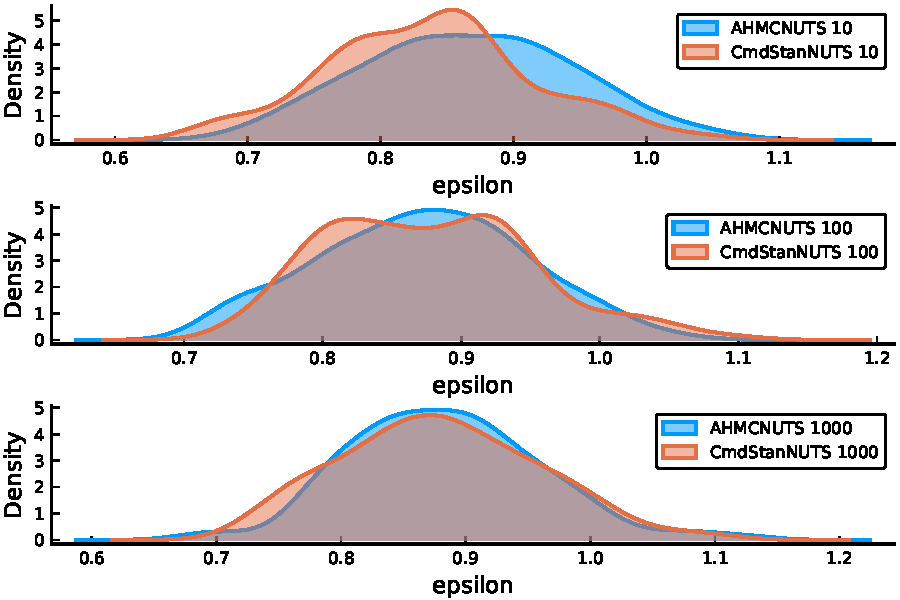
\includegraphics[width=0.08\textwidth]{./figs/SDT/density_epsilon.pdf}
        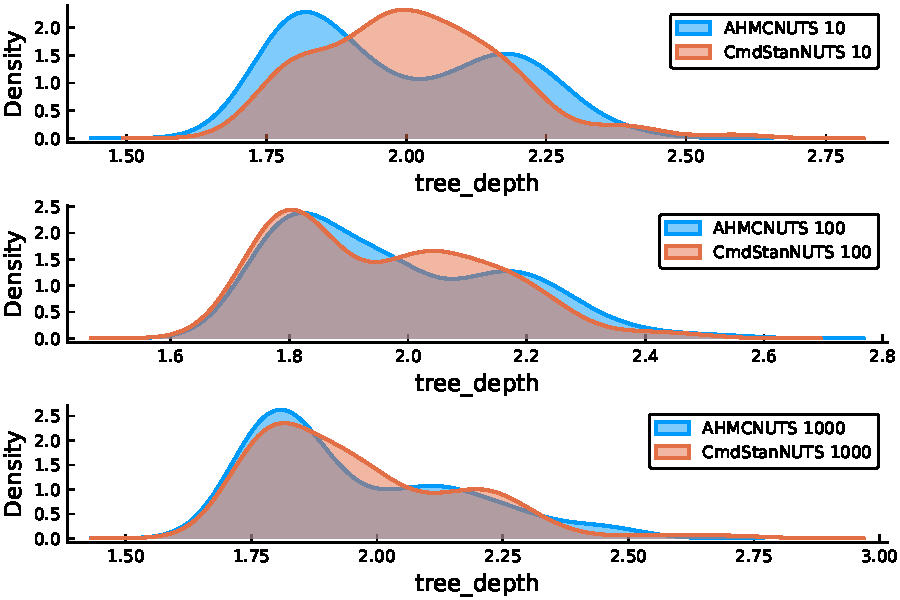
\includegraphics[width=0.08\textwidth]{./figs/SDT/density_tree_depth.pdf}
        \;\hfill
        \raisebox{\height}{\scalebox{0.75}{
            \begin{tabular}{lrrr}
                \toprule
                \multirow{2}{*}{} & \multirow{2}{*}{$N$} & \multicolumn{2}{c}{ESS} \\
                & & \multicolumn{1}{c}{$d$} & \multicolumn{1}{c}{$c$} \\
                \midrule
                \texttt{Stan} & 10 & 710.762  & 703.327 \\
                \texttt{AHMC} & 10 & 802.236 & 815.929 \\
                \texttt{Stan} & 100 & 820.741 & 823.152 \\
                \texttt{AHMC} & 100 & 814.308 & 846.357 \\
                \texttt{Stan} & 1000 & 844.478 & 872.961 \\
                \texttt{AHMC} & 1000 & 829.792 & 859.018 \\
                \bottomrule
            \end{tabular}
        }}\hfill\;
    \end{tikzfigure}
    \vspace{-2em}
    \begin{tikzfigure}[LR (50 runs); left to right: step size, tree depth, ESS]
        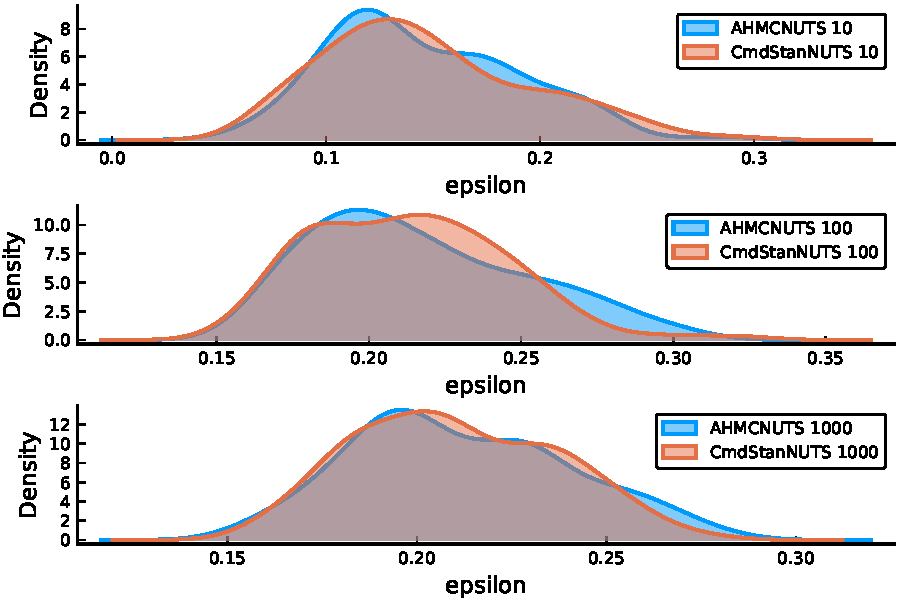
\includegraphics[width=0.08\textwidth]{./figs/Linear_Regression/density_epsilon.pdf}
        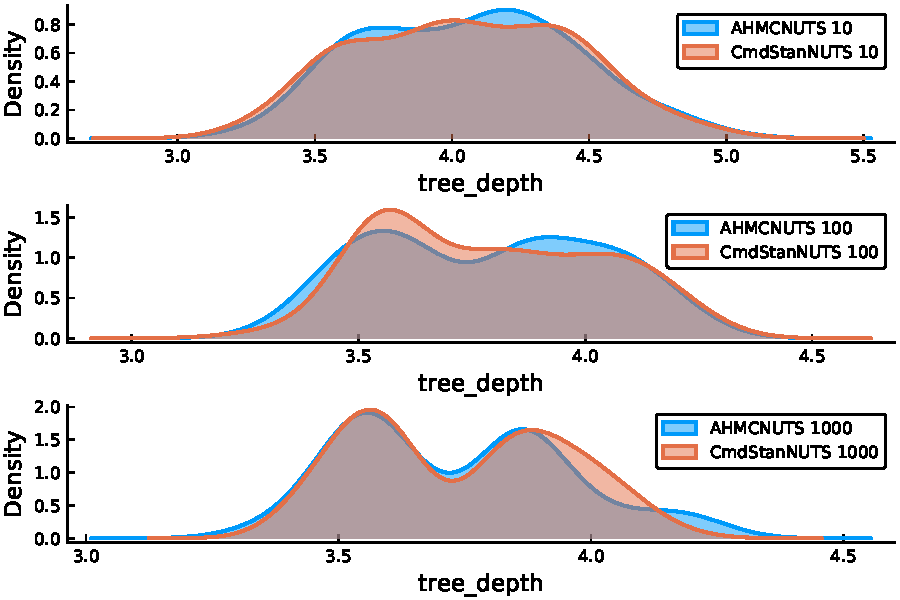
\includegraphics[width=0.08\textwidth]{./figs/Linear_Regression/density_tree_depth.pdf}
        \;\hfill
        \raisebox{\height}{\scalebox{0.75}{
            \begin{tabular}{lrrrrr}
                \toprule
                \multirow{2}{*}{} & \multirow{2}{*}{$N$} & \multicolumn{4}{c}{ESS} \\
                & & \multicolumn{1}{c}{$b_0$} & \multicolumn{1}{c}{$\sigma$} & \multicolumn{1}{c}{$b_1$} & \multicolumn{1}{c}{$b_2$} \\
                \midrule
                \texttt{Stan} & 10 & 413.939 & 266.476 & 381.219 & 423.441 \\
                \texttt{AHMC} & 10 & 354.946 & 263.894 & 411.769 & 399.420 \\
                \texttt{Stan} & 100 & 621.796 & 729.812 & 465.990 & 608.608 \\
                \texttt{AHMC} & 100 & 473.005 & 734.189 & 606.996 & 621.543 \\
                \texttt{Stan} & 1000 & 668.524 & 789.987 & 464.459 & 648.201 \\
                \texttt{AHMC} & 1000 & 485.988 & 786.577 & 676.097 & 689.344 \\
                \bottomrule
            \end{tabular}
        }}\hfill\;
    \end{tikzfigure}
    \vspace{-2em}
    \begin{tikzfigure}[HPR (25 runs); left to right: step size, tree depth, ESS (of some variables)]
        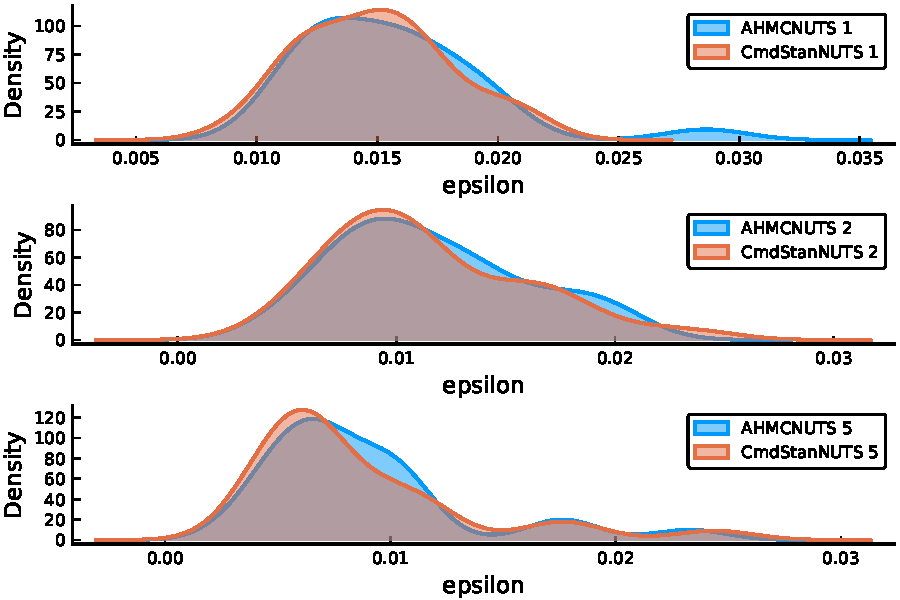
\includegraphics[width=0.08\textwidth]{./figs/Hierarchical_Poisson/density_epsilon.pdf}
        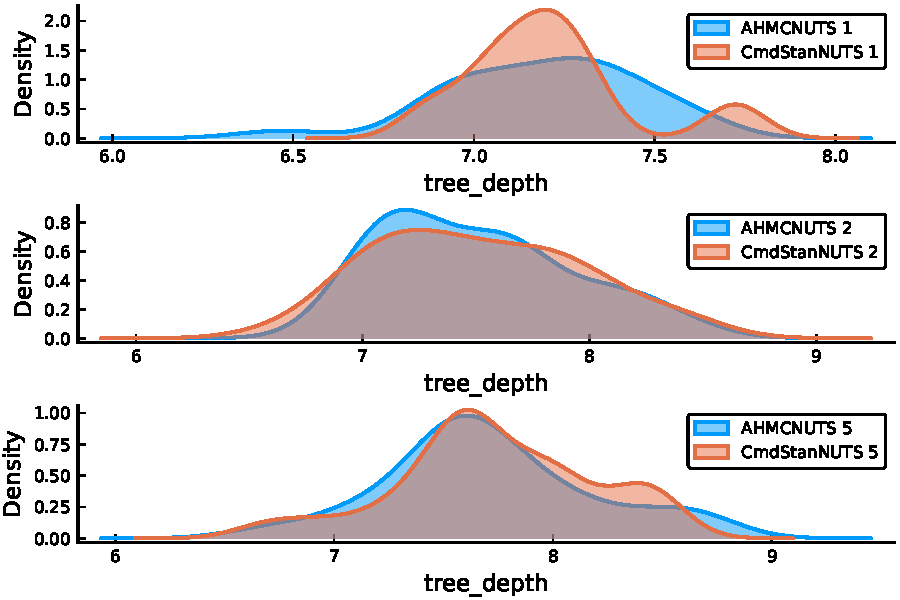
\includegraphics[width=0.08\textwidth]{./figs/Hierarchical_Poisson/density_tree_depth.pdf}
        \;\hfill
        \raisebox{\height}{\scalebox{0.75}{
            \begin{tabular}{lrrrr}
                \toprule
                \multirow{2}{*}{} & \multirow{2}{*}{$N$} & \multicolumn{3}{c}{ESS} \\
                & & \multicolumn{1}{c}{$a_0$} & \multicolumn{1}{c}{$a_1$} & \multicolumn{1}{c}{$b_\sigma$} \\
                \midrule
                \texttt{Stan} & 10 & 221.485 & 215.013 & 266.900 \\
                \texttt{AHMC} & 10 & 216.491 & 214.459 & 258.638 \\
                \texttt{Stan} & 20 & 208.286 & 207.041 & 241.080 \\
                \texttt{AHMC} & 20 & 206.458 & 200.469 & 236.546 \\
                \texttt{Stan} & 50 & 172.484 & 172.982 & 216.586 \\
                \texttt{AHMC} & 50 & 200.755 & 201.548 & 247.384 \\
                \bottomrule
            \end{tabular}
        }}\hfill\;
    \end{tikzfigure}
    \vspace{-2em}
    \begin{tikzfigure}[LBA (50 runs); left to right: step size, tree depth, ESS (of some variables)]
        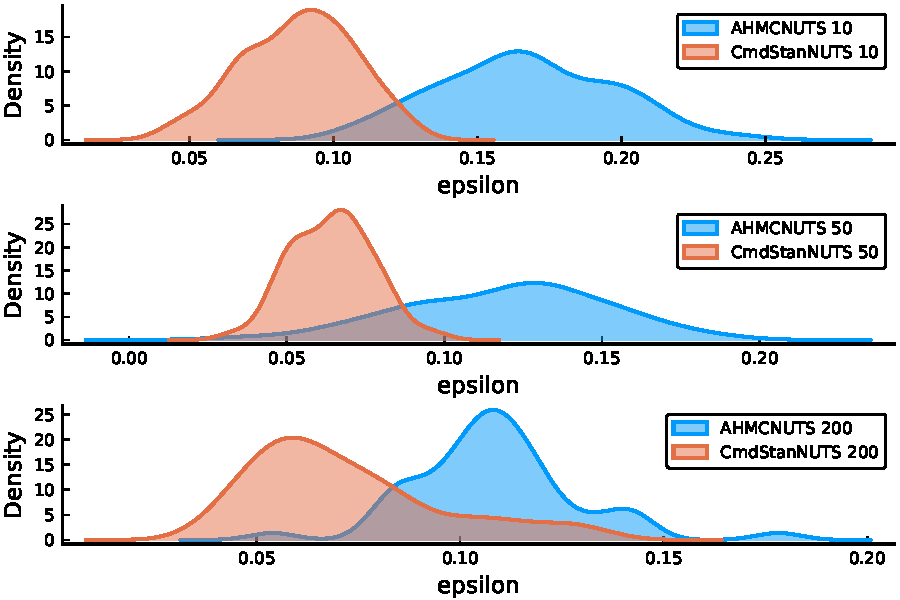
\includegraphics[width=0.08\textwidth]{./figs/LBA/density_epsilon.pdf}
        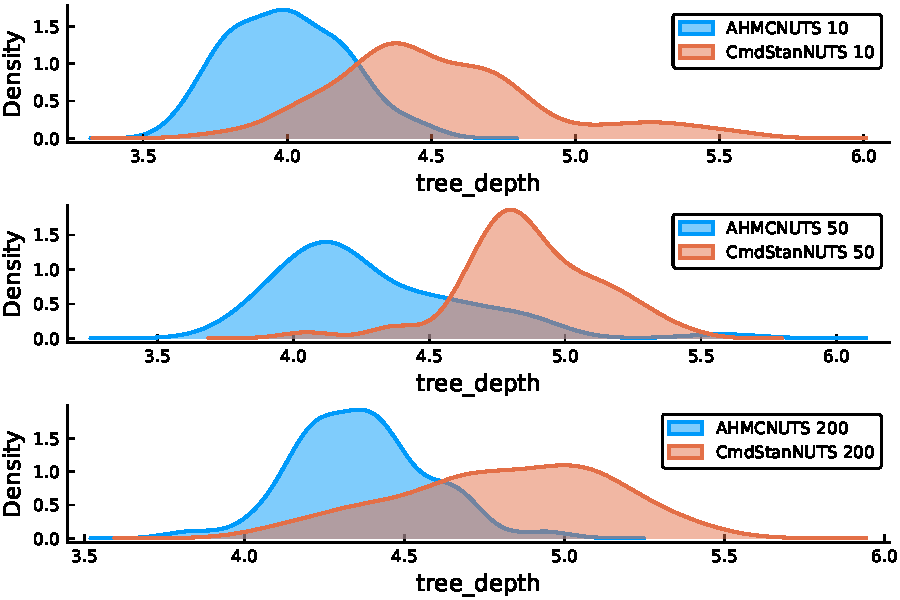
\includegraphics[width=0.08\textwidth]{./figs/LBA/density_tree_depth.pdf}
        \;\hfill
        \raisebox{\height}{\scalebox{0.75}{
            \begin{tabular}{lrrrrr}
                \toprule
                \multirow{2}{*}{} & \multirow{2}{*}{$N$} & \multicolumn{4}{c}{ESS} \\
                & & \multicolumn{1}{c}{$\tau$} & \multicolumn{1}{c}{$A$} & \multicolumn{1}{c}{$\nu_1$} & \multicolumn{1}{c}{$\nu_2$} \\
                \midrule
                \texttt{Stan} & 10 & 226.463 & 282.656 & 305.614 & 276.557 \\
                \texttt{AHMC} & 10 & 340.722 & 304.523 & 337.610 & 336.357 \\
                \texttt{Stan} & 50 & 212.838 & 238.003 & 235.009 & 232.667 \\
                \texttt{AHMC} & 50 & 248.249 & 238.979 & 248.331 & 255.421 \\
                \texttt{Stan} & 200 & 244.926 & 264.967 & 268.793 & 270.36 \\
                \texttt{AHMC} & 200 & 256.638 & 263.098 & 270.978 & 266.769 \\
                \bottomrule
            \end{tabular}
        }}\hfill\;
    \end{tikzfigure}
}

\npdecimalsign{.}
%\nprounddigits{5}

\column{0.32}
\block{Computational Efficiency: \texttt{Stan} v.s. \texttt{Turing}}{
    \texttt{Turing.jl} is a probabilistic programming language (PPL) in Julia that
    uses \texttt{AdvancedHMC.jl} as its HMC backend.
    All the benchmark models are written in \texttt{Turing} and \texttt{AdvancedHMC.jl}
    is called by \texttt{Turing.jl} to run the NUTS.
    Below is an example of running NUTS on the LR model using \texttt{Turing}.
    \lstinputlisting{lr.jl}    
    The time to run the five benchmark models in \texttt{Stan} and \texttt{Turing}
    are reported in the table below.
    \begin{tikztable}[Time comparisons between \texttt{Stan} and \texttt{Turing} (\texttt{AHMC}) for five models using $^1$ 25 runs, $^2$ 50 runs or $^3$ 100 runs.]
    \scalebox{0.9}{
    \begin{tabular}{lrrrrrrrrrr}
        \toprule
        %\multirow{2}{*}{} & \multicolumn{10}{c}{Data Size \& Mean Time (s)} \\
        & \multicolumn{2}{c}{Gaussian $^2$} & \multicolumn{2}{c}{SDT $^3$} & \multicolumn{2}{c}{LR $^2$} & \multicolumn{2}{c}{HPR $^1$} & \multicolumn{2}{c}{LBA $^2$} \\
        & \multicolumn{1}{c}{$N$} & \multicolumn{1}{c}{seconds} & \multicolumn{1}{c}{$N$} & \multicolumn{1}{c}{seconds} & \multicolumn{1}{c}{$N$} & \multicolumn{1}{c}{seconds}& \multicolumn{1}{c}{$N$} & \multicolumn{1}{c}{seconds}& \multicolumn{1}{c}{$N$} & \multicolumn{1}{c}{seconds} \\
        \midrule
        %\texttt{Stan} & 10 & 0.803881 & 10 & 0.775959 & 10 & 0.866924 & 10 & 2.487 & 10 & 1.91799 \\
        \texttt{Stan} & 10 & 0.8039 & 10 & 0.7759 & 10 & 0.8669 & 10 & 2.4870 & 10 & 1.9179 \\
        %Turing & 10 & 0.336073 & 10 & 0.328538 & 10 & 1.13563 & 10 & 19.4587 & 10 & 2.69062 \\
        \texttt{AHMC} & 10 & 0.3361 & 10 & 0.3285 & 10 & 1.1356 & 10 & 19.4587 & 10 & 2.6906 \\
        %\texttt{Stan} & 100 & 0.756092 & 100 & 0.726106 & 100 & 0.982419 & 20 & 3.50248 & 50 & 7.84705 \\
        \texttt{Stan} & 100 & 0.7561 & 100 & 0.7261 & 100 & 0.9824 & 20 & 3.5025 & 50 & 7.8471 \\
        %Turing & 100 & 0.33034 & 100 & 0.320111 & 100 & 1.32024 & 20 & 28.2982 & 50 & 11.027 \\
        \texttt{AHMC} & 100 & 0.3303 & 100 & 0.3201 & 100 & 1.3202 & 20 & 28.2982 & 50 & 11.0270 \\
        %\texttt{Stan} & 1000 & 0.761393 & 1000 & 0.708934 & 1000 & 2.26 & 50 & 5.89541 & 200 & 31.3762 \\
        \texttt{Stan} & 1000 & 0.7614 & 1000 & 0.7089 & 1000 & 2.2600 & 50 & 5.8954 & 200 & 31.3762 \\
        %Turing & 1000 & 0.508123 & 1000 & 0.317854 & 1000 & 3.83261 & 50 & 40.0322 & 200 & 33.6125 \\
        \texttt{AHMC} & 1000 & 0.5081 & 1000 & 0.3179 & 1000 & 3.8326 & 50 & 40.0322 & 200 & 33.6125 \\
        \bottomrule
    \end{tabular}
    }
    \end{tikztable}
    \vspace{-1em}
}

\block{Easy Integration of Other Julia Packages}{
    \texttt{Bijectors.jl} is used inside \texttt{Turing.jl} to do automatic transformations of constrained variables to run HMC.
    E.g. a random variable from $\mathcal{T}runcated(\mathcal{C}auchy(0, 5), 0, \infty)$ is constrained to be positive and 
    will be transformed to the real space by the $\log$ function automatically. \\
    
    \texttt{CuArrays.jl} could be used with \texttt{AdvancedHMC.jl} to run NUTS on GPUs.
    In order to run NUTS using CUDA, 
    one only needs to change Line 3 of the demo code 
    from \texttt{q\_init = randn(D)} to \texttt{q\_init = CuArray(randn(D))}, 
    assuming \texttt{logdensity\_f} and \texttt{grad\_f} in Line 6 are GPU friendly;
    if it is written in pure Julia, it probably supports GPUs acceleration automatically. \\
    \textit{How does it work?}
   All arrays in \texttt{AdvancedHMC.jl} are abstractly typed, meaning that the concrete type is deduced at compile time from \texttt{q\_init}. That is to say, if \texttt{q\_init} is on the GPU i.e. is a CuArray, all the internal arrays in the NUTS will be too. \\

    \texttt{SoSS.jl} is another PPL in Julia that
    uses \texttt{AdvancedHMC.jl} as its backend.
    It is easy for PPLs in Julia with different domain specific languages (DSLs)
    to use the HMC implementation in \texttt{AdvancedHMC.jl}. \\

    \texttt{DifferentialEquations.jl} is the state-of-the-art numerical differential equations solver package, implemented in pure Julia. As such, its solvers can be employed in Turing models, thus enabling \texttt{AHMC} to perform Bayesian inference in the parameters of differential equation models. \\

    \texttt{Flux.jl} is a deep learning packages in Julia.
    Neural models defined by \texttt{Flux.jl} can be directly used in Turing models.
    E.g. one can implement a Bayesian neural network in Turing by 
    defining priors on the weights of a Flux-based neural network, and 
    NUTS can be used to draw samples of the weights.
}

\block{Acknowledgements}{
    We would like to thank the developers of \texttt{MCMCBenchmarks.jl}, Rob Goedman and Christopher Fisher.
    With this package we ran all benchmarks and generated all plots presented in this poster.
    % We would also like to thank Martin Trapp for useful discussions on efficient implementations of the benchmark models in Turing.jl.
}

\block{References}{
    \vspace{-1em}
    {\footnotesize \printbibliography[heading=none]}
}
    
\end{columns}
\end{document}